\documentclass{template/socthesis}

\usepackage{subcaption}
\usepackage{amsmath}
\usepackage{enumitem}

\addbibresource{text.bib}

\titlecz{Budík na platforme Arduino}
\titleen{X}
\author{Kristína Rybárová\\Matej Hrachovec}
\field{11}
\school{Gymnázium Brno, třída kpt.~Jaroše}
\mentor{doc. PhDr. Jana Nováková, Ph.D.}
\mentorstatement{doc. PhDr. Jany Novákové, Ph.D.}

% Změňte, pokud se liší
\region{Trenčiansky samosprávny kraj}
\placefooter{Trenčín 2020}

\begin{document}

\maketitle

\makecopyrightstatement{V Trenčíne}

\pagestyle{plain}

\tableofcontents % vysází obsah

%%% Začátek práce
\setcounter{figure}{0}
\setcounter{table}{0}
\newpage

\chapter*{Úvod}
\addcontentsline{toc}{chapter}{Úvod} % přidá položku úvod do obsahu
Platforma Arduino umožnuje blablabbla... Rozhodli sme sa vytvoriť jednoduchý budík, ktorý demonštruje možnosti tejto platformy.

\newpage

\chapter{Teoretické východiská}

\section{Arduino}
Arduino je open-source platforma používaná na vytváranie elektronických projektov. Samotná platforma pozostáva z fyzickej, programovateľnej vývojovej dosky pripojiteľnej typicky cez USB a vývojového prostredia pre počítače~\cite{maly-hvj}.

Pod názvom Arduino bolo vytvorených množstvo verzií vývojových dosiek, v našej práci sa zameriame na verziu Arduino Uno (Rev3).

\subsection{Arduino Uno}
Jadrom dosky Arduino Uno je mikrokontrolér ATmega328P pracujúci na frekvencii 16 MHz. Samotná doska obsahuje 14 digitálnych (z toho 6 PWM) a 6 analógových vývodov. Taktiež obsahujuje 32 kB flash pamäte, 2 kB pamäte SRAM a 1 kB pamäte EEPROM~\cite{arduino-uno}.

\begin{figure}
    \centering
    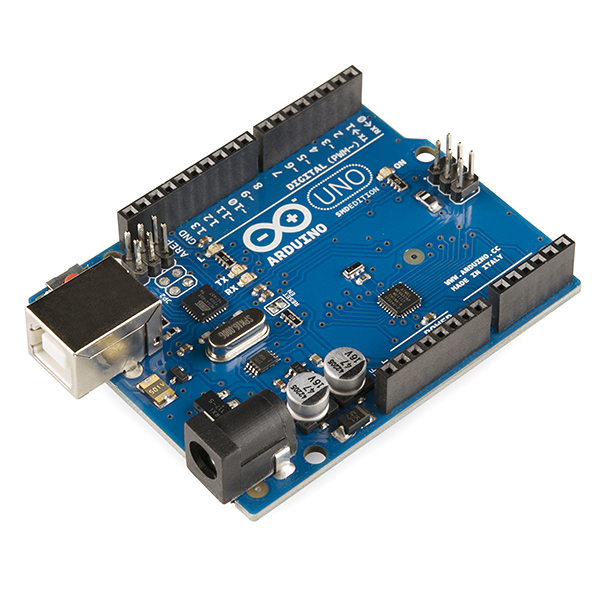
\includegraphics{img/Arduino_Uno.jpg}
    \caption{Arduino Uno.}
\end{figure}

\subsection{Vývojové prostredie}
Pre vývoj programov je primárne určené vývojové prostredie Arduino IDE. Podporuje vývoj v jazykoch C a C++ a obsahuje štandardnú knižnicu z projektu Wiring~\cite{maly-hvj}.

\begin{figure}
    \centering
    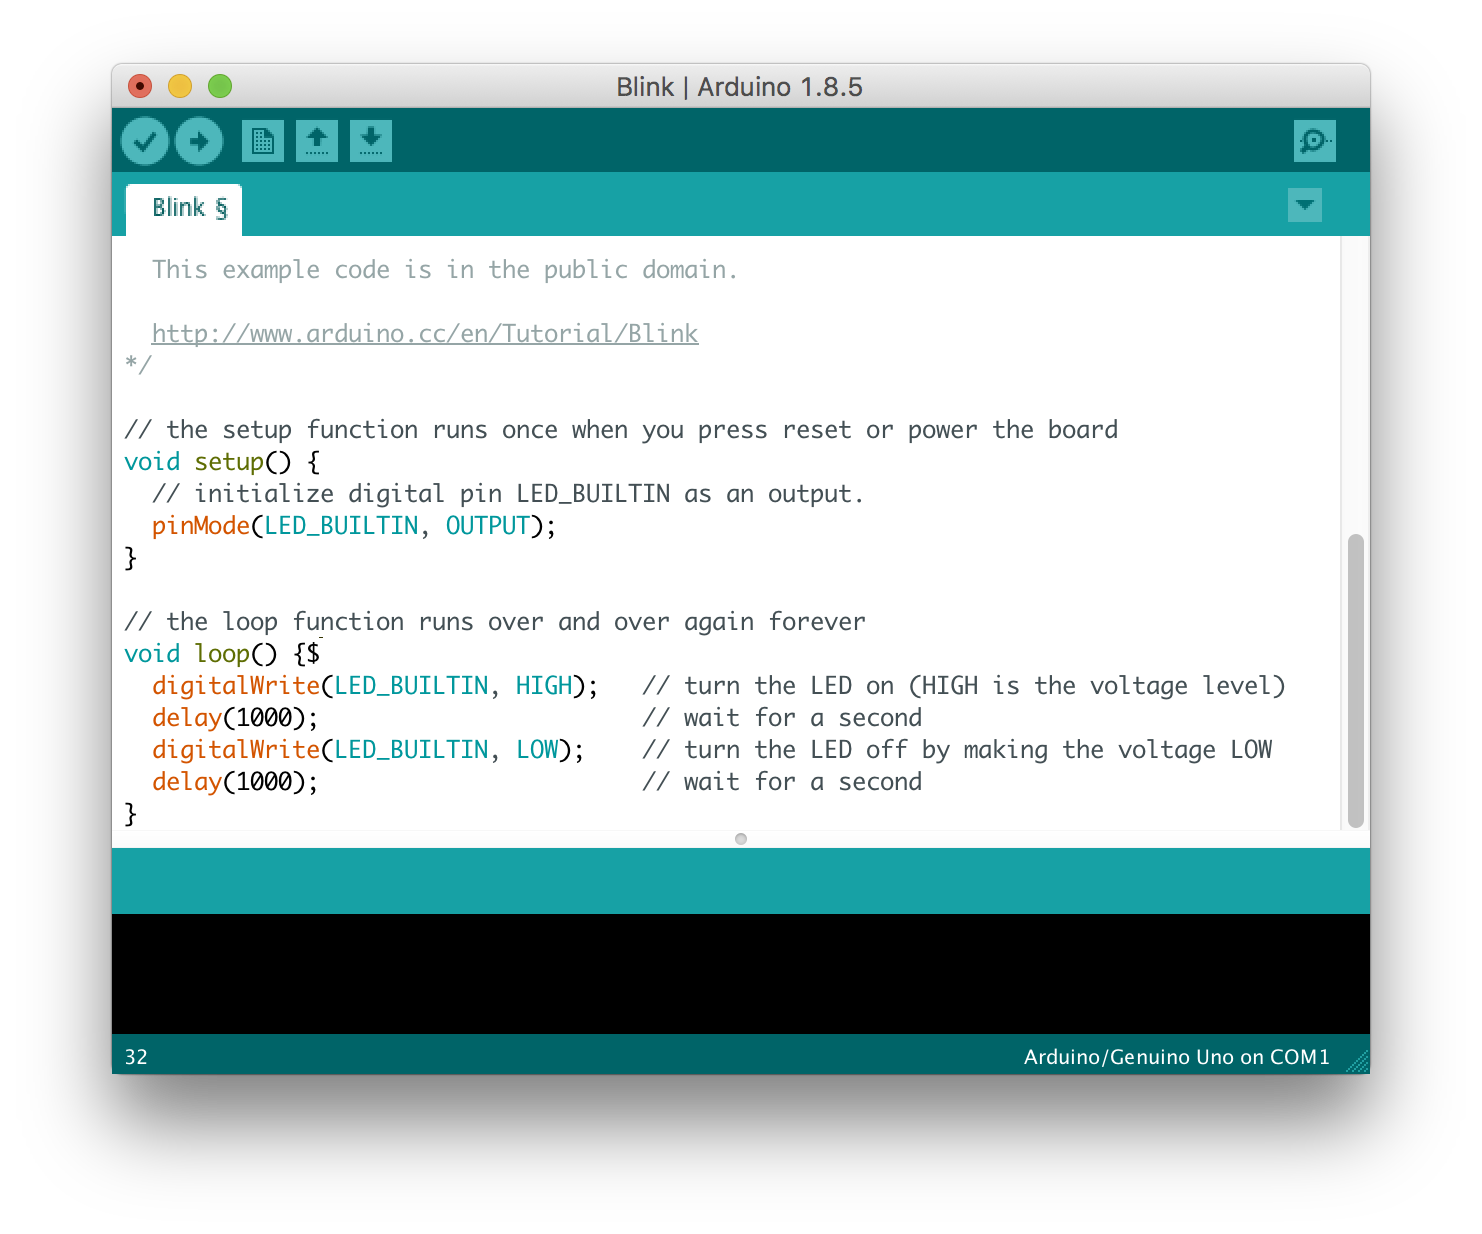
\includegraphics[width=\textwidth]{img/Arduino_IDE.png}
    \caption{Vývojové prostredie Arduino IDE.}
\end{figure}

Programovanie pre Arduino má niektoré odlišnosti oproti bežnému programovaniu v C/C++. Samotný program sa v Arduino terminológií nazýva \emph{sketch} a musí obsahovať 2 funkcie: jednu pre inicializáciu (\texttt{void setup()}) a druhá obsahuje hlavný cyklus programu (\texttt{void loop()})~\cite{maly-hvj}.

\section{Modul reálneho času}
Nakoľko pre budík je udržovanie presného údaju o aktuálnom čase kriticky dôležité, je vhodné využiť pre tento účel modul reálneho času (RTC). Jedná sa o integrovaný obvod ktorý sleduje skutočný čas nezávisle od ostatných súčastí systému~\cite{rtc-adafruit}. Vďaka zálohovacej batérií funguje aj pri strate hlavného napájania.

Hardvér samotného Arduina RTC neobsahuje, je však možné ho jednoducho pripojiť.
%\section{LCD Display}

\chapter{Ciele práce}
Hlavným cieľom našej práce bolo vyrobiť budík na platforme Arduino Uno. Budík by mal v štandardnom režime ukazovať dátum, čas a teplotu. V zvolenom čase budík zvukovo upozorní. Stíšiť budík je možné iba zadaním hesla, ktoré môže uživateľ nastaviť.

Na dosiahnutie toho je nutné naštudovanie platformy Arduino Uno, výber vhodných komponentov, navrhnutie a zapojenie obvodu a naprogramovanie riadiaceho programu.

\chapter{Metodika práce}

\section{Výber komponentov}
Cieľovú platformu Arduino Uno sme samozrejme museli doplniť ďalšímí komponentmi, ktoré umožňujú realizáciu nášho zadania.

Okrem spomínaného RTC modulu sme pre komunikáciu s používateľom použili 16x2 LCD displej a 4x4 membránovú klávesnicu. Ďalej sme použili piezomenič na vydanie akustického tónu.

\subsection{Zoznam použitých komponentov}
\begin{itemize}
    \item Arduino Uno
    \item RTC modul DS3231
    \item LCD displej LCD1602
    \item membránová klávesnica ER-CCO21601C
    \item piezomenič
    \item potenciometer \SI{10}{\kilo\ohm}
    \item rezistor \SI{220}{\ohm}
\end{itemize}

\section{Návrh zapojenia}
Celkové zapojenie sme navrhli na základe odporúčaných postupov pre jednotlivé komponenty. Vývody na doske Arduino sme volili tak, aby boli súvisiace komponenty zapojené spolu, no v niektorých prípadoch toto nebolo možné vzhľadom na vlastnosti niektorých vývodov (napr. PWM).

Pre realizáciu obvodu sme dočasne využili nepájivé pole. Do budúcnosti je plánované umiestniť hotový výrobok do krabičky.

\section{Implementácia}
Pri programovaní sme použili programovací jazyk C++ a vhodné knižice pre prácu so zvolenými komponentmi.

Po spustení sa inicializuje RTC, pričom ak sa jedná o prvé spustenie po programovaní, tak sa čas kompilácie nastaví ako inicializačný čas, čím odpadá potreba ručne nastavovať čas. Taktiež prebehne inicializácia iných komponentov.

Následne sa v hlavnom cykle programu pravidelne zisťuje aktuálny čas z modulu RTC a porovnáva s časom budenia.

\chapter{Výsledky práce}
Vytvorili sme budík na platforme Arduino Uno s využitím modulu reálneho času a LCD displeja. Implementované riešenie spĺňa všetky požiadavky kladené v cieľoch práce a demonštuje nektoré možnosti zvolenej platformy.

Snažili sme sa tiež navrhnúť dostatočne jednoduché a intuitívne ovládanie vzhľadom na možnosti poskytnuté použitými komponentmi. Pre úplnosť je návod na použitie uvedený v nasledujúcej sekcii.

\section{Ovládanie}
V základnom režime budík zobrazuje dátum, čas a teplotu. Pri neaktivite sa stlmí podsvietenie displeja.

\vspace{5mm}
\begin{figure}[h]
    \centering
    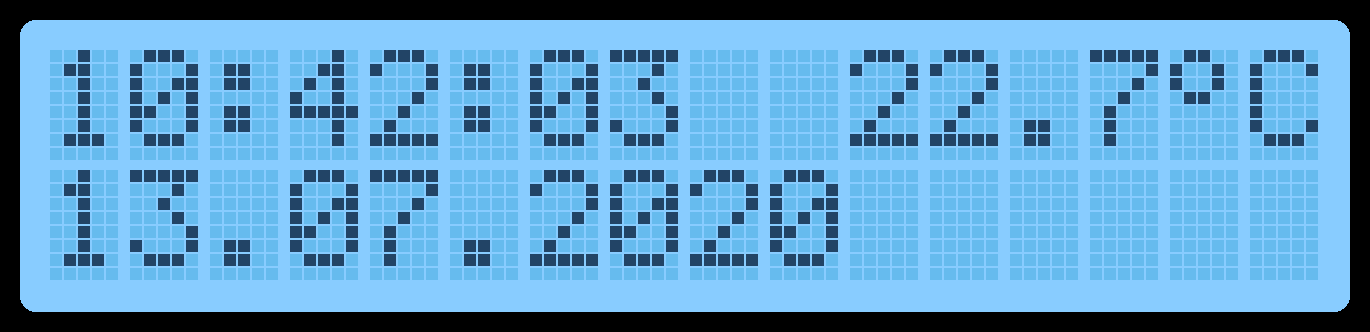
\includegraphics[width=0.7\textwidth]{img/display_time.png}
    \caption{Zobrazenie dátumu, času a teploty v základnom režime.}
\end{figure}

Pre nastavenie času budenia stlačíme tlačidlo \texttt{A}. Následne je možné tlačidlami zadať požadovaý čas budenia a potvrdiť tlačidlom \texttt{\#}.

\vspace{5mm}
\begin{figure}[h]
    \centering
    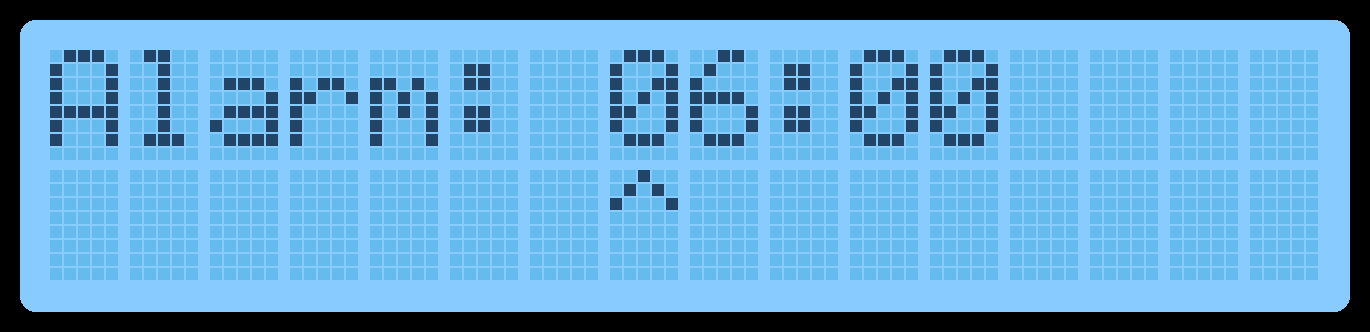
\includegraphics[width=0.7\textwidth]{img/display_set_alarm.png}
    \caption{Nastavenie času budenia.}
\end{figure}

\clearpage

Vo zvolenom čase budík začne budiť hlasným tónom a na displeji sa zobrazí výzva na zadanie hesla. Heslo je možné zadať tlačidlami a potvrdiť tlačidlom \texttt{\#}. Ak je heslo správne, budík sa stíši, v opačnom prípade bude zvoniť ďalej.

\vspace{5mm}
\begin{figure}[h]
    \centering
    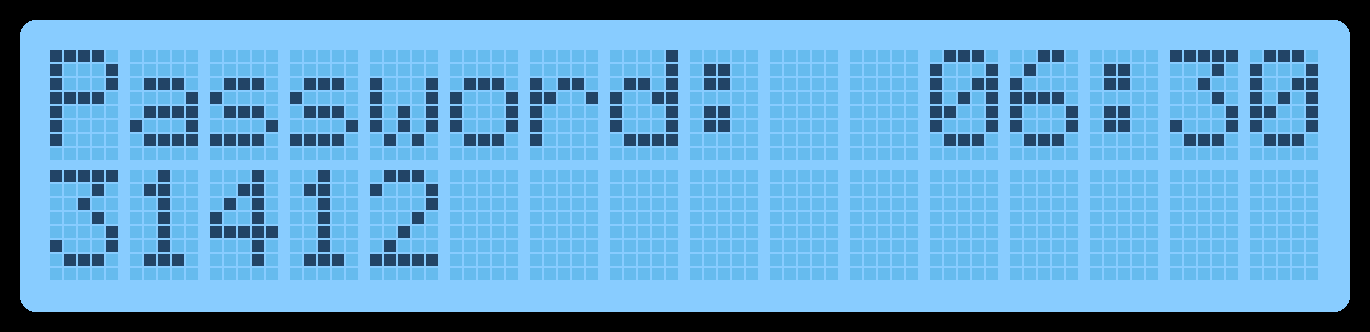
\includegraphics[width=0.7\textwidth]{img/display_alarm.png}
    \caption{Budenie.}
\end{figure}

Pre nastavenie vlastného hesla stlačíme tlačidlo \texttt{B}. Následne je možné tlačidlami zadať nové heslo a potvrdiť tlačidlom \texttt{\#}.

\vspace{5mm}
\begin{figure}[h]
    \centering
    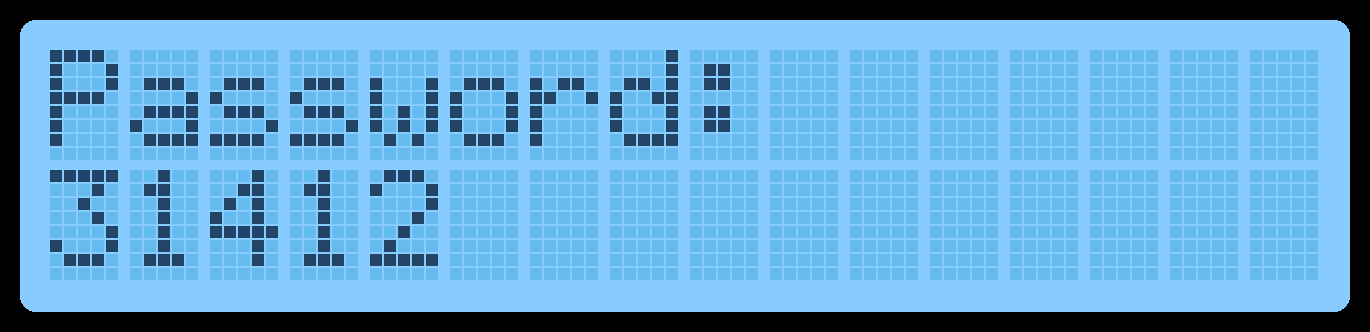
\includegraphics[width=0.7\textwidth]{img/display_set_pass.png}
    \caption{Nastavenie hesla.}
\end{figure}

\chapter*{Záver}
\addcontentsline{toc}{chapter}{Záver}

Závěrečná kapitola obsahuje zhodnocení dosažených výsledků se zvlášť vyznačeným vlastním přínosem studenta.
Povinně se zde objeví i zhodnocení z~pohledu dalšího vývoje projektu, student uvede náměty vycházející ze zkušeností s~řešeným projektem a uvede rovněž návaznosti na právě dokončené projekty.

\begingroup
\vspace{20mm}
\let\clearpage\relax
\chapter*{Conclusion}
\addcontentsline{toc}{chapter}{Conclusion}
\endgroup
Asdf

\newpage


\printbibliography[title=Zoznam použitej literatúry]
\addcontentsline{toc}{chapter}{Zoznam použitej literatúry}

%\listoffigures
%\addcontentsline{toc}{section}{Seznam obrázků}

%\listoftables
%\addcontentsline{toc}{section}{Seznam tabulek}

%\listoflistedequation
%\addcontentsline{toc}{section}{Seznam rovnic}

\end{document}
